\documentclass[format=sigconf]{acmart}
\usepackage[utf8]{inputenc}
\usepackage{geometry}
\usepackage{enumitem}
\usepackage{float}
\usepackage[labelfont=bf,textfont=md]{caption}
\usepackage{graphicx}
\usepackage{xcolor}
\usepackage{minted}
\usepackage{hyperref}
\usepackage[parfill]{parskip}
\usepackage[all]{hypcap}
\usemintedstyle[common-lisp]{default}
\newmintinline[code]{text}{}
\bibliographystyle{plainnat}

\hypersetup{
  colorlinks,
  linkcolor={red!50!black},
  citecolor={blue!50!black},
  urlcolor={blue!80!black}
}

\newlist{step}{enumerate}{10}
\setlist[step]{label*=\arabic*.,leftmargin=2em}

\acmConference[ELS’25]{the 18th European Lisp Symposium}
{May 19--20 2025}{Zürich, Switzerland}
\acmDOI{}
\setcopyright{rightsretained}
\copyrightyear{2025}

\begin{document}

\title{Porting the Steel Bank Common Lisp Compiler and Runtime to the Nintendo Switch NX Platform}

\author{Charles Zhang}
\email{charleszhang99@yahoo.com}
\author{Yukari ``Shinmera'' Hafner}
\email{shinmera@tymoon.eu}
\affiliation{%
  \institution{Shirakumo.org}
  \city{Zürich}
  \country{Switzerland}
}

\begin{CCSXML}
<ccs2012>
   <concept>
       <concept_id>10011007.10011006.10011041.10011048</concept_id>
       <concept_desc>Software and its engineering~Runtime environments</concept_desc>
       <concept_significance>500</concept_significance>
       </concept>
   <concept>
       <concept_id>10011007.10011006.10011041.10011045</concept_id>
       <concept_desc>Software and its engineering~Dynamic compilers</concept_desc>
       <concept_significance>500</concept_significance>
       </concept>
   <concept>
       <concept_id>10011007.10010940.10010941.10010949.10010950.10010954</concept_id>
       <concept_desc>Software and its engineering~Garbage collection</concept_desc>
       <concept_significance>300</concept_significance>
       </concept>
   <concept>
       <concept_id>10011007.10011074</concept_id>
       <concept_desc>Software and its engineering~Software creation and management</concept_desc>
       <concept_significance>100</concept_significance>
       </concept>
 </ccs2012>
\end{CCSXML}

\ccsdesc[500]{Software and its engineering~Runtime environments}
\ccsdesc[500]{Software and its engineering~Dynamic compilers}
\ccsdesc[300]{Software and its engineering~Garbage collection}
\ccsdesc[100]{Software and its engineering~Software creation and management}

\begin{abstract}
  The Nintendo Switch (NX) is a 64-bit ARM-based platform for video games with a proprietary micro-kernel operating system. Notably this system does not give programs the ability to mark pages as executable or give access to thread signal handlers, both of which present a significant hurdle to SBCL's intended bootstrap process and runtime operation. We present our efforts to adapt the SBCL runtime and compiler to deploy applications onto the NX platform.
\end{abstract}

\keywords{Common Lisp, SBCL, porting, ARM, aarch64, NX, Experience Report}

\maketitle

\def\abovecaptionskip{1pt}
\def\listingautorefname{Listing}
\def\figureautorefname{Figure}

\section{Introduction}\label{introduction}
The Nintendo Switch (codename NX) is a handheld video game console based on the ARM 4 Cortex-A57 64-bit architecture\cite{morgan2020}. It features a proprietary micro-kernel operating system called the ``Nintendo Switch system software''\cite{roussel2019methodically} (NX OS), and normally only runs software that has been licensed, approved, and digitally signed and encrypted by Nintendo.

Developing licensed software for the NX has to be done via Nintendo's own proprietary SDK, which they only distribute under a non-disclosure agreement (NDA). An open-source third-party alternative to the SDK is available\cite{switchbrew}, but this cannot be used for licensed software.

The OS-provided runtime environment is only directly suitable for C and C++ software. Other game engines such as Unity, Unreal, and Godot do provide exporting functionality to the NX, meaning that ports for the runtime environments they rely on such as C\#, Lua, and GDScript have been developed, but remain closed-source.

A port of a C-based runtime for Common Lisp such as ECL\cite{attardi1994embeddable} is conceivable. However, due to the high performance requirements of video games and the relatively low-power platform of the NX, we deemed it unlikely for such a port to lead to a useful platform. Besides, relying on a C runtime would not eliminate all the difficulties we've encountered in porting SBCL anyway.

Particularly, every known Common Lisp implementation compiles a part of its runtime from Lisp source code incrementally into itself, and all user-code is also incrementally compiled into the Lisp image, as opposed to being batch-compiled and linked like other languages such as C. We cannot incrementally compile code on the NX due to platform security restrictions. The consequence is that all implementation and all user code needs to be compiled ahead of time. We discuss the intricacies of this in \autoref{build} and \autoref{relocation}.

The NX OS further does not provide user signal handlers. This is a problem for the Garbage Collector (GC), as SBCL relies on inter-thread signalling to park threads during garbage collection. While SBCL does provide a safepoints mechanism for GC that is used on Windows, this mechanism had not been tested on any other platform, and as-is still did not meet the requirements of this locked-down platform. We discuss the GC in detail in \autoref{gc}.

While we can now compile and deploy complex Common Lisp applications to the NX, some parts of the runtime remain unsupported, and we discuss our future efforts in this regard in \autoref{further-work}.

\section{Related Work}\label{relatedwork}
Rhodes\cite{rhodes2008sbcl} outlines the methodology behind the SBCL bootstrapping process.

A pure Common Lisp bootstrapping process as Durand et al.\cite{durand2019bootstrapping} outline would however not notably improve our process, as all our challenges arise from not being able to bootstrap on the desired target platform in the first place, and needing to handle the low-level system construction processes to be amenable for the NX' restrictions.

Citing information on the NX' operating system is difficult as it is a closed-source platform with all usual information placed under NDA. All publicly available information is from security research such as by Roussel-Tarbouriech et al.\cite{roussel2019methodically} and reverse-engineering\cite{switchbrew}.

Particularly, we are unaware of any publication about the porting of other runtime environments to the NX, such as C\#, JavaScript, Lua, etc.

Patton\cite{patton2023parallel} and Schwartz\cite{schwartz2018dynamic} describe some details about SBCL's garbage collector which we modify for our port.

\section{Build System}\label{build}
The usual SBCL build process proceeds in several distinct phases, some of which need to be run on a ``host system'' and others on the ``target system''. This does allow for limited cross-compilation, wherein the ``host system'' steps can be run on an operating system and platform that is not that of the target we are trying to compile for. However, the ``target system'' steps cannot currently be performed on a host system, and full incremental code execution is required on the target. As mentioned in the Introduction, we cannot perform incremental code execution on the NX, as the NX OS does not allow us to map new executable pages.

The basic idea of our solution to this issue is to replace the NX as \textit{initial} target with an ARM64-based Linux. Once everything, including user code, has been compiled on this Linux target, we extract all Lisp code and data out using a process called \textit{shrinkwrapping} and link it together with the SBCL C runtime as compiled for the NX. This process ultimately results in a fully static ELF executable that does not perform any dynamic memory mapping or compilation.

Our build still functions largely the same as the one outlined by Rhodes\cite{rhodes2008sbcl}, though being run roughly twice with special configurations to accomplish the hybrid build.

\begin{enumerate}
\item \code{build-config} (NX) \\
  This step gathers whatever build configuration options for the target and spits them out into a readable format for the rest of the build process. We run this on some host system (which may not be our ARM64 Linux intermediary), using a special flag to indicate that we're building for the NX. We also enable the fasteval contrib, which we need to step in for any place where we would usually invoke the compiler at runtime.
\item \code{make-host-1} (NX) \\
  Next we build the cross-compiler with the host Lisp compiler, and at the same time emit C header files describing Lisp object layouts in memory as C structs for the next step.
\item \code{make-target-1} (NX) \\
  Now we use the C compiler the Nintendo SDK provides for us, which can cross-compile the SBCL C runtime for the NX. We had to make adjustments to the C runtime bits, as the NX OS is not POSIX compliant and lacks a few features the SBCL C runtime usually takes advantage of. The SBCL C runtime contains the GC and OS glue bits that the Lisp code needs.
\item \code{build-config} (Linux$\sim$NX) \\
  We now create an almost-normal ARM64 Linux system with the same feature set as for the NX. This involves the usual steps as before, though with a special flag to inform some parts of the Lisp process that we're going to ultimately target the NX.
\item \code{make-host-1} (Linux$\sim$NX)
\item \code{make-target-1} (Linux$\sim$NX)
\item \code{make-host-2} (Linux$\sim$NX)
  With the target runtime built, we build the target Lisp system (compiler and the standard library) using the Lisp cross-compiler built by the Lisp host compiler in \code{make-host-1} (Linux). This step produces a "cold core" that the runtime can jump into, and can be done purely on the host machine. This cold core is not complete, and needs to be executed on the target machine with the target runtime to finish bootstrapping, notably to initialise the object system, which requires runtime compilation.
\item \code{make-target-2} (Linux$\sim$NX) \\
  The cold core produced in the last step is loaded into the target runtime, and finishes the bootstrapping procedure to compile and load the rest of the Lisp system. After the Lisp system is loaded into memory, the memory is dumped out into a "warm core", which can be loaded back into memory in a new process with the target runtime. From this point on, new code can be loaded and images can be dumped at will.
\item \code{user} \\
  For user code we now perform some tricks to make it think it's running on the NX, rather than on Linux. In particular we modify \code{*features*} to include \code{:nx} and not \code{:linux}, \code{:unix}, or \code{:posix}. Once that is set up and ASDF has been neutered, we can compile our program "as usual" and at the end dump out a new core.
\item \code{shrinkwrap} \\
  Once all our code has been loaded and a final core has been produced, we ``shrinkwrap'' the image to produce assembly files. The details of this are outlined in \autoref{relocation}. These assembly files can then be linked together with the SBCL C runtime compiled for the NX in step (3) with the Nintendo SDK toolchain, producing a final ELF executable.
\item \code{package} \\
  The final step is to run all the other SDK toolchain bits to produce a signed application package, which can be deployed to a Nintendo Switch development kit to be run.
\end{enumerate}

A notable extra wrinkle in this procedure is that the SDK is only available for Windows. To accommodate this, the custom build system we developed can be run either directly from Windows using another ARM machine remotely to run the Linux bits, or it can be run from a Linux system with the ARM bits being run either locally or remotely and the Windows bits being run either remotely or through Wine\cite{amstadt1994wine}.

\section{Relocation}\label{relocation}

\colorbox{red}{
  \textbf{TODO CHARLES}: Add some details here.
}

\section{Garbage Collection}\label{gc}
SBCL' default garbage collector, ``gencgc'', is a stop-the-world collector. In order to start collecting, it needs to ``park'' all threads in a safe location where they won't access any memory that the collector might move or change during collection.

On Unix systems signals are used to park the threads. By sending a signal to every other thread, each thread will enter a signal handler, which can then park the thread. This is advantageous, since it leverages an operating system mechanism to interrupt thread execution and frees the thread from checking whether it should park.

On Windows no equivalent mechanism is available, so a technique called ``safepoints'' is employed instead. The compiler injects code at strategic locations, such as at function call boundaries and loop returns, which checks whether the thread should park explicitly. This strategy is notably slower than using signals, since the safepoints are not free, and is finicky, as the compiler could inject too many safepoints (slowing execution of user code significantly) or too few safepoints (making threads take too long to park).

In order to make the safepoint test as small and cheap as possible SBCL does employ another trick on Windows: each safepoint simply writes to a memory region. When GC is triggered, this region is marked as protected, causing any thread that tries to write to it to trap, which SBCL can intercept to park the thread instead.

On the NX we cannot install trap handlers, so the current safepoint strategy fails.

\colorbox{red}{
  \textbf{TODO CHARLES}: Add some details here.
}

\section{Conclusion}\label{conclusion}
We have demonstrated that it is possible to port SBCL even to a very restrictive platform that is hostile towards dynamic runtimes such as used for Lisp.

\begin{figure}[h]
  \centering
  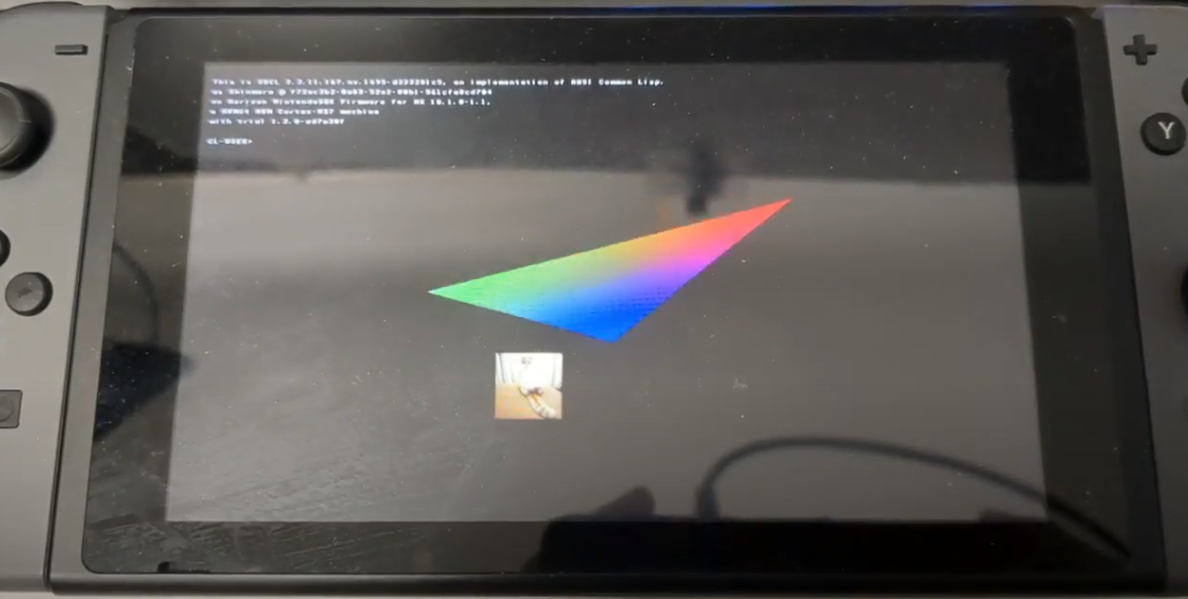
\includegraphics[width=\linewidth]{photo.png}
  \caption{A photo of a demo running in the Trial Common Lisp game engine on the Nintendo Switch hardware.}
\end{figure}

Using a substitute build host that is similar enough to the target platform we can compile all code ahead of time, then substitute the base runtime and rewrite the resulting code in order to create an executable suitable for the target platform.

We have also managed to update the garbage collector to work on operating systems with more restrictive feature sets than are found on a typical desktop operating system.

\section{Further Work}\label{further-work}
Currently we rely on the fasteval system to circumvent runtime compilation restrictions. This is especially vital for CLOS, since the discriminating function is only compiled on first call of a generic function. However, since we know that we don't dynamically add or remove methods, we should be able to pre-compile all of these functions as well. We'd like to add such a CLOS freeze step to the build pipeline.

Callbacks from C to Lisp are currently left unimplemented. Callbacks in SBCL are implemented in part as hand-written assembly stubs, and are very hard to maintain. The current stubs for ARM64 do not work correctly in the presence of the shrinkwrapping steps that we make use of.

Finally there are a number of improvements we've made that we would like to upstream to lessen the maintenance burden. We've already contributed a bunch of the changes back upstream, but a lot of it is also tied to the proprietary SDK and cannot be open-sourced due to the NDA, and some other changes are too contentious for the rest of the SBCL team to want to upstream.

\section{Acknowledgements}\label{acknowledgements}
We would like to thank Douglas Katzman for his help and advice for various parts of the porting effort, as well as the rest of the SBCL maintenance team for their continuous improvements to the SBCL platform.

\bibliography{paper}

\end{document}

%%% Local Variables:
%%% mode: latex
%%% TeX-command-extra-options: "-shell-escape"
%%% TeX-master: t
%%% TeX-engine: luatex
%%% End:
